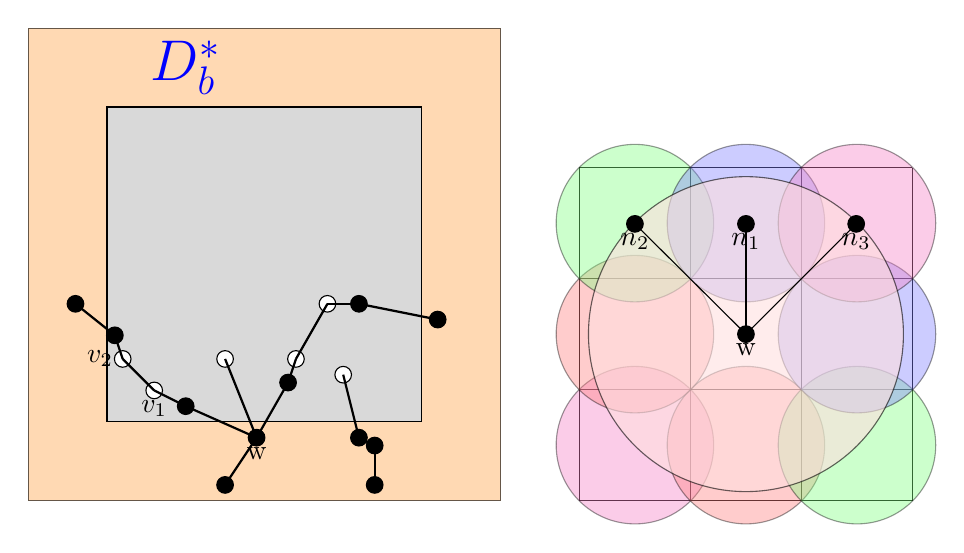
\begin{tikzpicture}

    % Square in the middle
    
    \draw[ fill=orange!50, opacity=0.6] (2, 2) rectangle ++(6, 6);
    \draw[ fill=gray!30] (3, 3) rectangle ++(4, 4);

    

    \coordinate (v6) at (4.9, 2.8);

    \filldraw[fill=black] (v6) circle (3pt) node[below]{w};

    \coordinate (v72) at (4.5, 2.2);

    \filldraw[fill=black] (v72) circle (3pt);

    \coordinate (v9b) at (6.2, 2.8);

    \filldraw[fill=black] (v9b) circle (3pt);

    \coordinate (v9c) at (6.4, 2.7);

    \filldraw[fill=black] (v9c) circle (3pt);

    \coordinate (v9d) at (6.4, 2.2);

    \filldraw[fill=black] (v9d) circle (3pt);

    \coordinate (v92) at (7.2, 4.3);

    \filldraw[fill=black] (v92) circle (3pt);

    \coordinate (v5) at (4.5, 3.8);

    \filldraw[fill=white] (v5) circle (3pt);

    \coordinate (v71) at (5.3, 3.5);

    \filldraw[fill=black] (v71) circle (3pt);

    \coordinate (v73) at (5.4, 3.8);

    \filldraw[fill=white] (v73) circle (3pt);

    \coordinate (v10) at (4, 3.2);

    \filldraw[fill=black] (v10) circle (3pt);

    \coordinate (v11) at (3.6, 3.4);

    \filldraw[fill=white] (v11) circle (3pt) node[below]{$v_1$};

    \coordinate (v12) at (3.2, 3.8);

    \filldraw[fill=white] (v12) circle (3pt) node[left]{$v_2$};

    \coordinate (v13) at (3.1, 4.1);

    \filldraw[fill=black] (v13) circle (3pt) ;

    \coordinate (v14) at (2.6, 4.5);

    \filldraw[fill=black] (v14) circle (3pt) ;
    

    

    

    

    \coordinate (v9a) at (6, 3.6);

    \filldraw[fill=white] (v9a) circle (3pt);

    \coordinate (v91) at (6.2, 4.5);

    \filldraw[fill=black] (v91) circle (3pt);

    \coordinate (v93) at (5.8, 4.5);

    \filldraw[fill=white] (v93) circle (3pt);

    

    

    

   \node at (4,7.5) {\huge{\textcolor{blue}{$D^*_b$}}};



    
    \draw [thick, black](v5) -- (v6);
    \draw [thick, black](v6) -- (v71);
    \draw [thick, black](v91) -- (v92);
    \draw [thick, black](v9a) -- (v9b);

   
    


    \draw [thick, black](v6) -- (v72);
    \draw [thick, black](v9b) -- (v9c);
    \draw [thick, black](v9c) -- (v9d);
    \draw [thick, black](v91) -- (v93);
    \draw [thick, black](v71) -- (v73);
    \draw [thick, black](v10) -- (v6);
    \draw [thick, black](v10) -- (v11);
    \draw [thick, black](v12) -- (v11);
    \draw [thick, black](v12) -- (v13);
    \draw [thick, black](v13) -- (v14);
    \draw [thick, black](v73) -- (v93);


    \begin{scope}[xshift= 9cm, yshift = 2cm]

        \draw[step = 1.41] (0, 0) grid (4.23, 4.23);
        \draw[fill = magenta!50, opacity = 0.4] (0.705, 0.705) circle (1);
        \draw[fill = red!50, opacity = 0.4] (2.115, 0.705) circle (1);
        \draw[fill = green!50, opacity = 0.4] (3.525, 0.705) circle (1);
        \draw[fill = red!50, opacity = 0.4] ( 0.705, 2.115) circle (1);
        \draw[fill = green!50, opacity = 0.4] ( 0.705, 3.525) circle (1);
        \draw[fill = blue!50, opacity = 0.4] ( 2.115, 3.525) circle (1);
        \draw[fill = blue!50, opacity = 0.4] ( 3.525, 2.115) circle (1);
        \draw[fill = magenta!50, opacity = 0.4] ( 3.525, 3.525) circle (1);
        \draw[fill = pink!50, opacity = 0.6] ( 2.115, 2.115) circle (2);

        \draw[fill = black] ( 2.115, 2.115) circle (3pt) node[below]{w};
        \draw[fill = black] ( 2.115, 3.515) circle (3pt);
        \draw[fill = black] ( 0.705, 3.515) circle (3pt);
        \draw[fill = black] ( 3.515, 3.515) circle (3pt);

        \draw[] ( 2.115, 2.115) -- ( 2.115, 3.515) node[below]{$n_1$};
        \draw[] ( 2.115, 2.115) -- ( 0.705, 3.515) node[below]{$n_2$};
        \draw[] ( 2.115, 2.115) -- ( 3.515, 3.515) node[below]{$n_3$};
        

        
    \end{scope}

    


    

\end{tikzpicture}

